\section{Getting started with Kali Linux}
\subsection{Activity}

\noindent {\bf{Bước 1:}} Truy cập vào đường dẫn \href{https://old.kali.org/kali-images/kali-2016.2/}{Link} và chọn phiên bản Kali Linux 2016 phù hợp rồi tải về.

\begin{figure}[!htb]
    \centering
    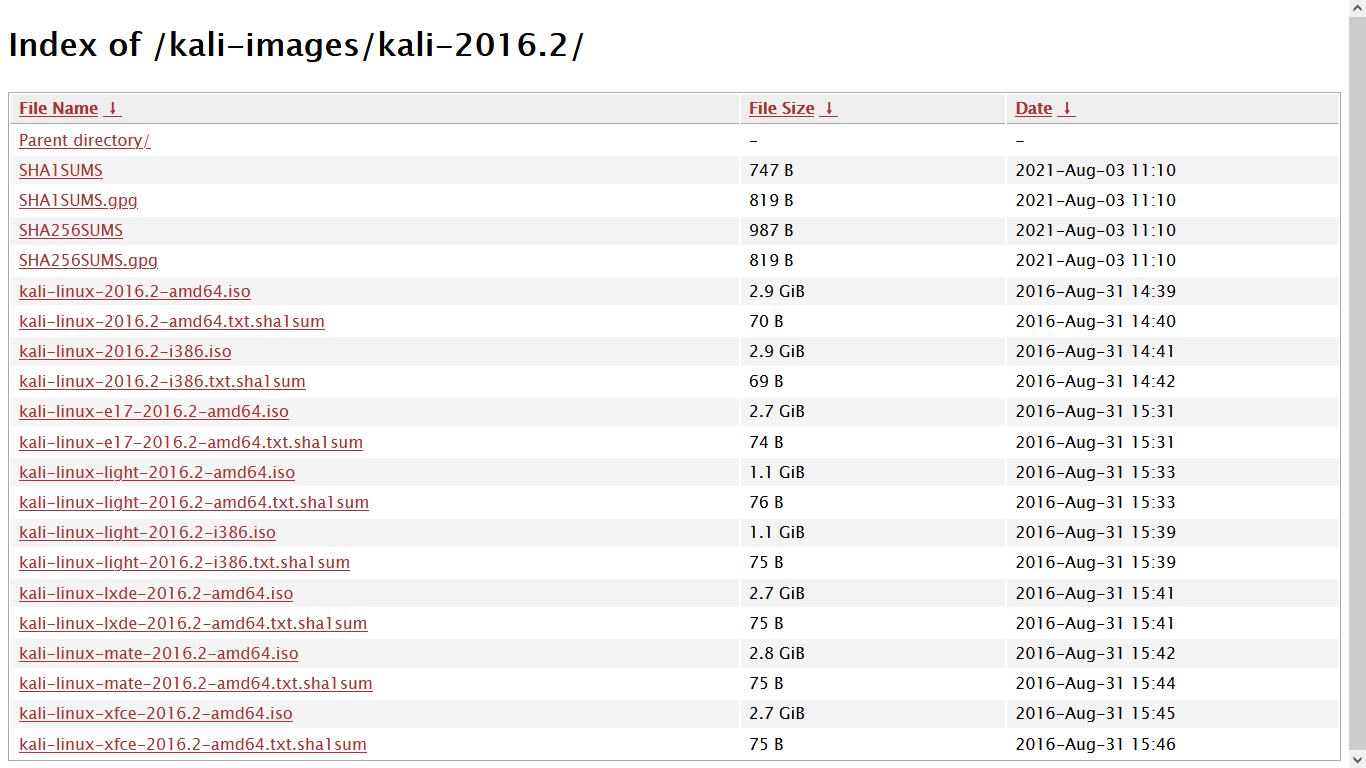
\includegraphics[width=0.9\linewidth]{figure//chapter5//lab5_1/download_kali_linux.png}
    \caption{Tải Kali Linux 2016}
    \label{fig:enter-label}
\end{figure}

\noindent {\bf{Bước 2:}} Cấu hình máy ảo và khởi động. Chọn máy ảo Linux, phiên bản Linux 2.6/3.x/4.x/5.x. Cấp 25GB bộ nhớ, 2 cpu. Tạo máy ảo và khởi động.

\begin{figure}[!htb]
    \centering
    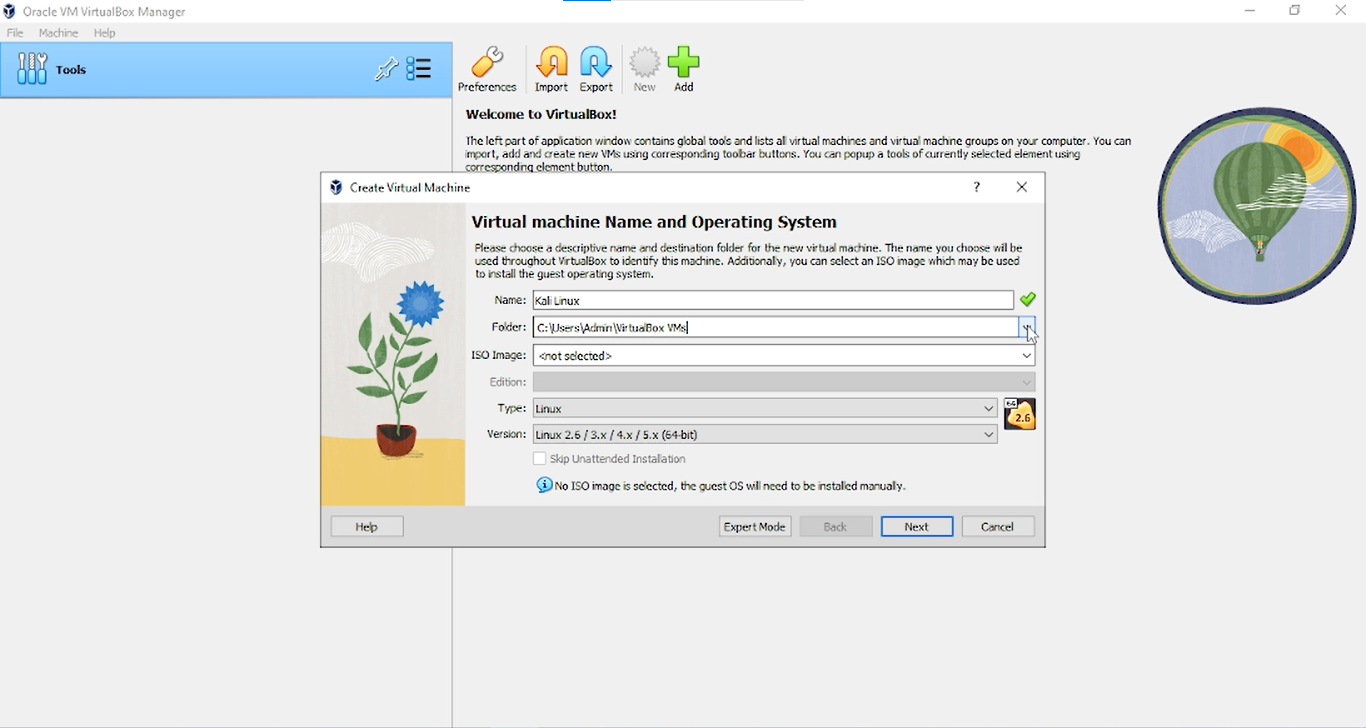
\includegraphics[width=0.9\linewidth]{figure//chapter5//lab5_1/create_vm.png}
    \caption{Tạo máy ảo}
    \label{fig:enter-label}
\end{figure}

\newpage

\noindent {\bf{Bước 3:}} Sau khi khởi động xong, chọn \textbf{Graphical Install}.

\begin{figure}[!htb]
    \centering
    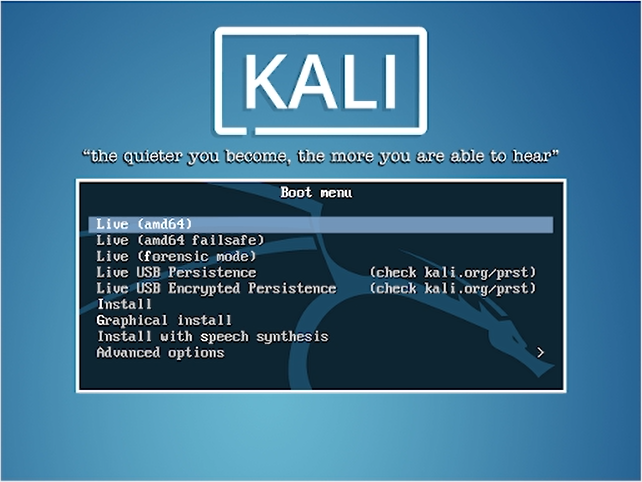
\includegraphics[width=0.85\linewidth]{figure//chapter5//lab5_1/graphical_install.png}
    \caption{Boot options}
    \label{fig:enter-label}
\end{figure}

\noindent {\bf{Bước 4:}} Tiếp tục với các cài đặt mặc định. Tại \textbf{Configure the network}, nhập \textbf{Test.com} và \textbf{Continue}. Sau đó nhập mật khẩu là \textbf{admin}.

\begin{figure}[!htb]
    \centering
    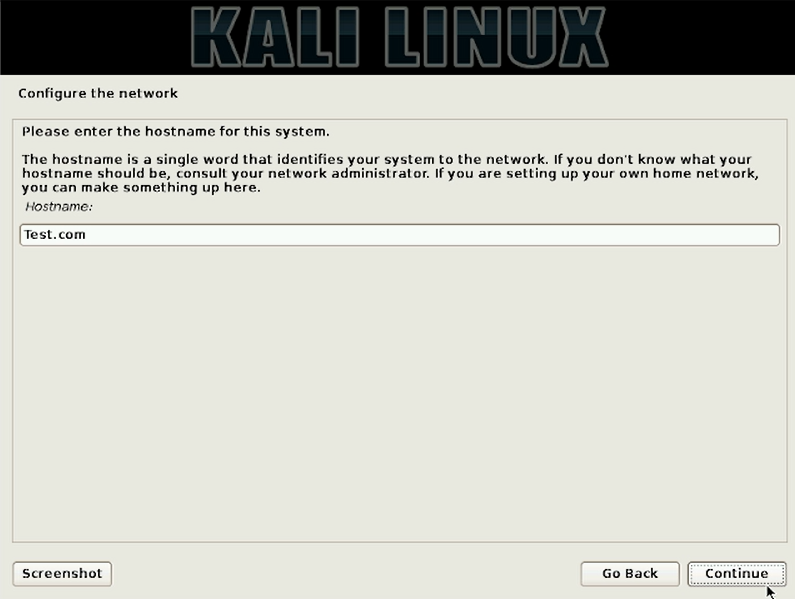
\includegraphics[width=0.85\linewidth]{figure//chapter5//lab5_1/configure_network.png}
    \caption{Cấu hình mạng}
    \label{fig:enter-label}
\end{figure}

\noindent {\bf{Bước 5:}} Tại \textbf{Partition disks}, chọn \textbf{Yes}.

\begin{figure}[!htb]
    \centering
    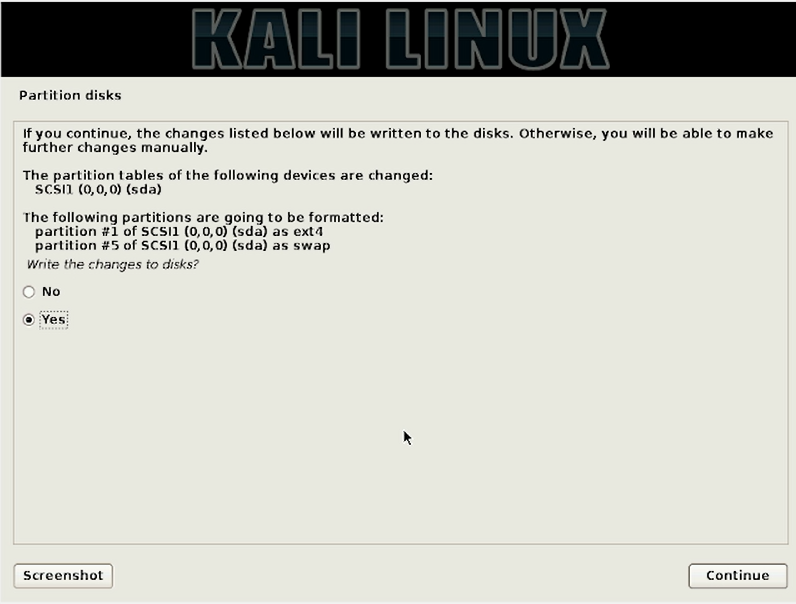
\includegraphics[width=0.85\linewidth]{figure//chapter5//lab5_1/partition_disk.png}
    \caption{Partition Disks Configuration}
    \label{fig:enter-label}
\end{figure}

\noindent {\bf{Bước 6:}} Tại \textbf{Configre the package manager}, chọn \textbf{No}.

\begin{figure}[!htb]
    \centering
    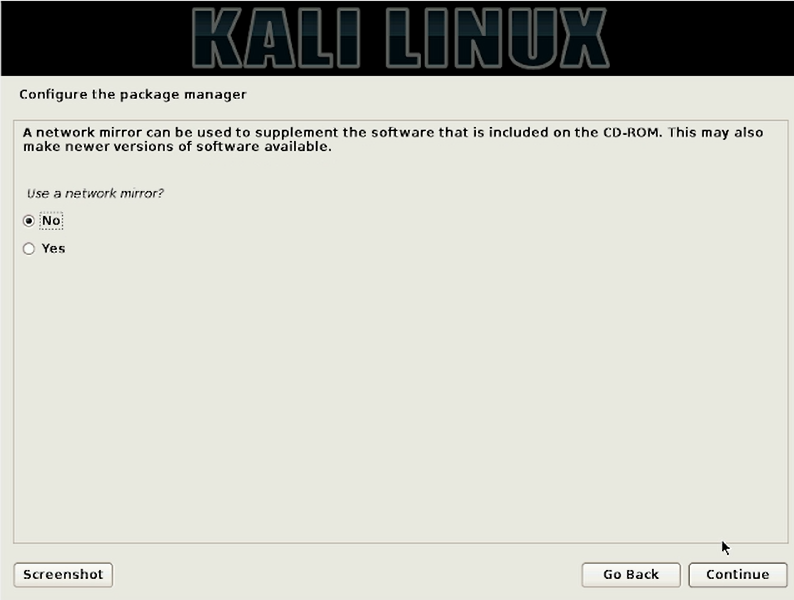
\includegraphics[width=0.85\linewidth]{figure//chapter5//lab5_1/package_manager.png}
    \caption{Package Manager Configuration}
    \label{fig:enter-label}
\end{figure}

\newpage

\noindent {\bf{Bước 7:}} Tại \textbf{GRUB boot loader}, chọn \textbf{Yes}. Sau đó chọn các cài đặt mặc định và \textbf{Install}. Cuối cùng khởi động lại máy.

\begin{figure}[!htb]
    \centering
    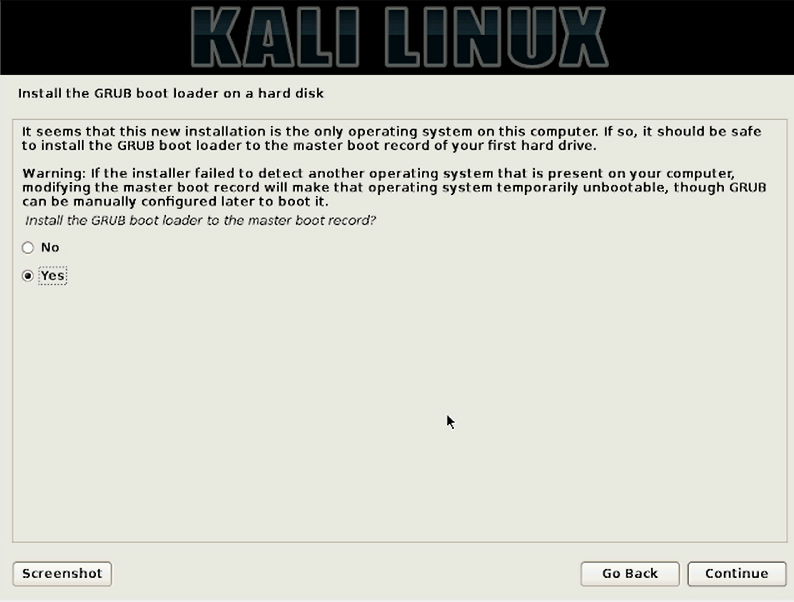
\includegraphics[width=0.85\linewidth]{figure//chapter5//lab5_1/GRUB.png}
    \caption{GRUB Boot Loader}
    \label{fig:enter-label}
\end{figure}

\noindent {\bf{Bước 8:}} Nhập \textbf{root} và \textbf{admin} để đăng nhập vào hệ thống.

\begin{figure}[!htb]
    \centering
    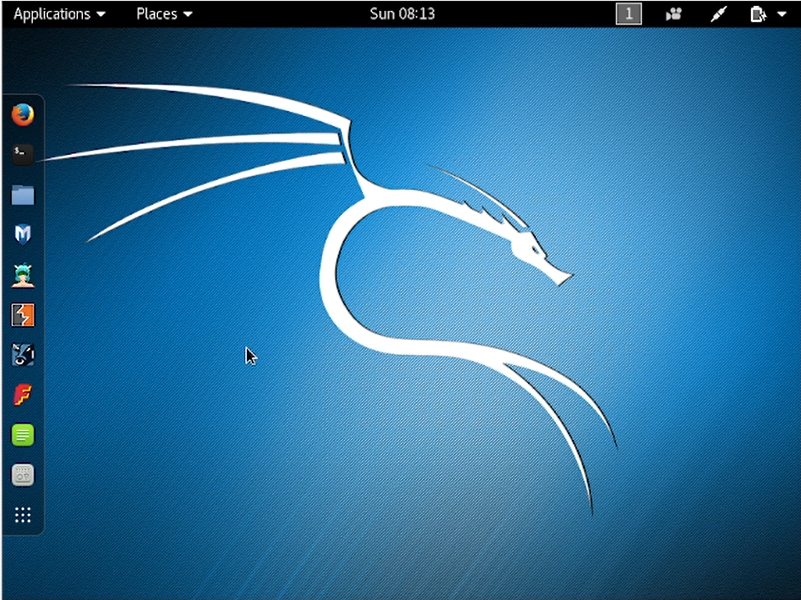
\includegraphics[width=0.85\linewidth]{figure//chapter5//lab5_1/login.png}
    \caption{Login to Linux}
    \label{fig:enter-label}
\end{figure}

\noindent {\bf{Bước 9:}} Mở \textbf{Terminal}.

\begin{figure}[!htb]
    \centering
    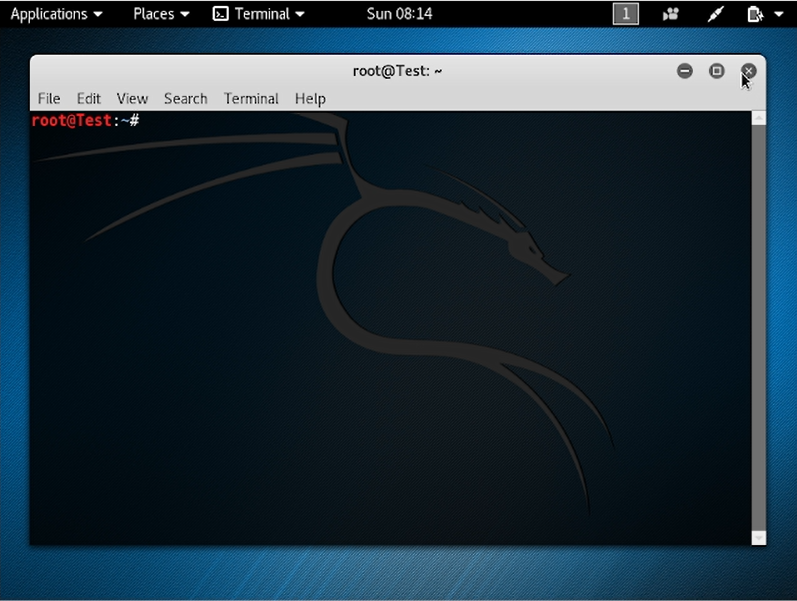
\includegraphics[width=0.85\linewidth]{figure//chapter5//lab5_1/terminal.png}
    \caption{Mở Terminal}
    \label{fig:enter-label}
\end{figure}

\noindent {\bf{Bước 10:}} Nhập \textbf{ifconfig}. Nếu inet addr bằng 127.0.0.1, thì tức là bạn phải cấu hình địa chỉ IP thủ công.

\begin{figure}[!htb]
    \centering
    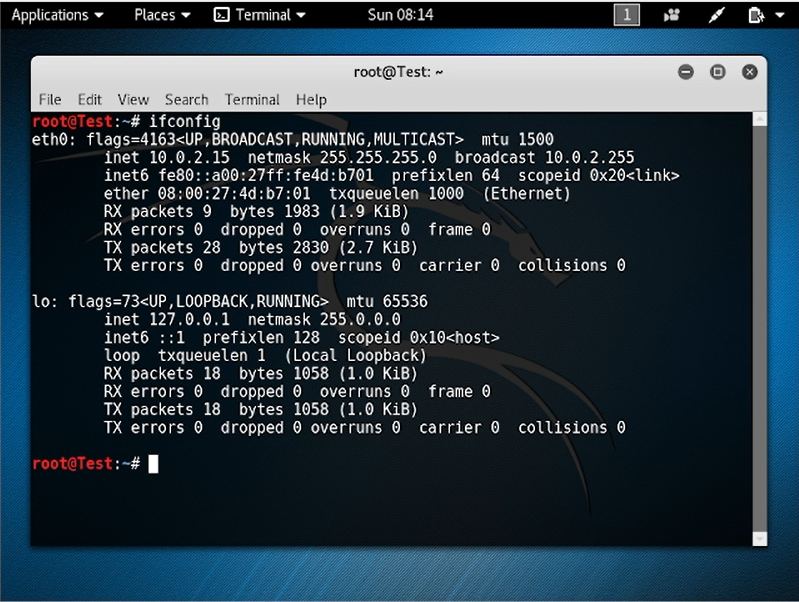
\includegraphics[width=0.85\linewidth]{figure//chapter5//lab5_1/manual_configure.png}
    \caption{Kết quả khi thực hiện ifconfig}
    \label{fig:enter-label}
\end{figure}

\newpage

\noindent {\bf{Bước 11:}} Nhập \textbf{/etc/init.d/networking start} để bắt đầu dịch vụ mạng.

\begin{figure}[!htb]
    \centering
    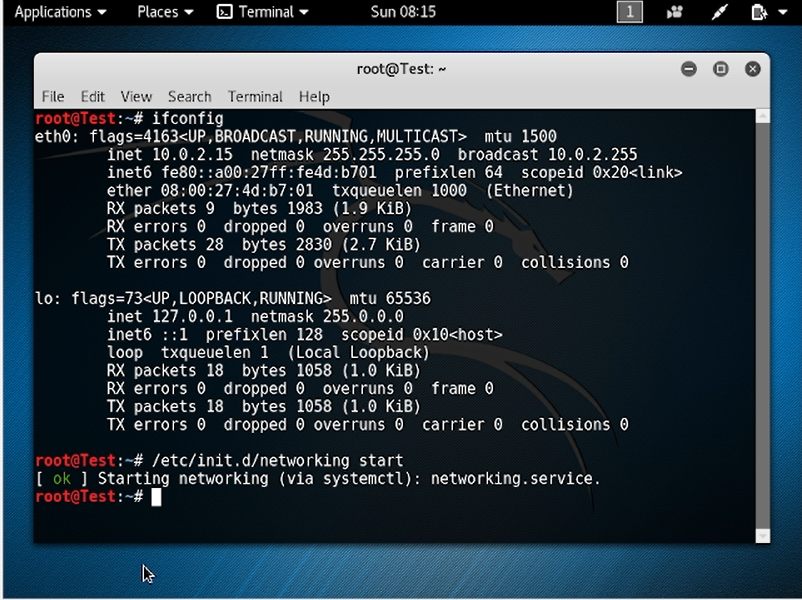
\includegraphics[width=0.85\linewidth]{figure//chapter5//lab5_1/networking_service.png}
    \caption{Khởi động dịch vụ mạng}
    \label{fig:enter-label}
\end{figure}

\noindent {\bf{Bước 12:}} Ở VirtualBox, chọn \textbf{Machine/Settings/Network}. Chắc VM đã nhận ra được Adapter của máy bạn.

\begin{figure}[!htb]
    \centering
    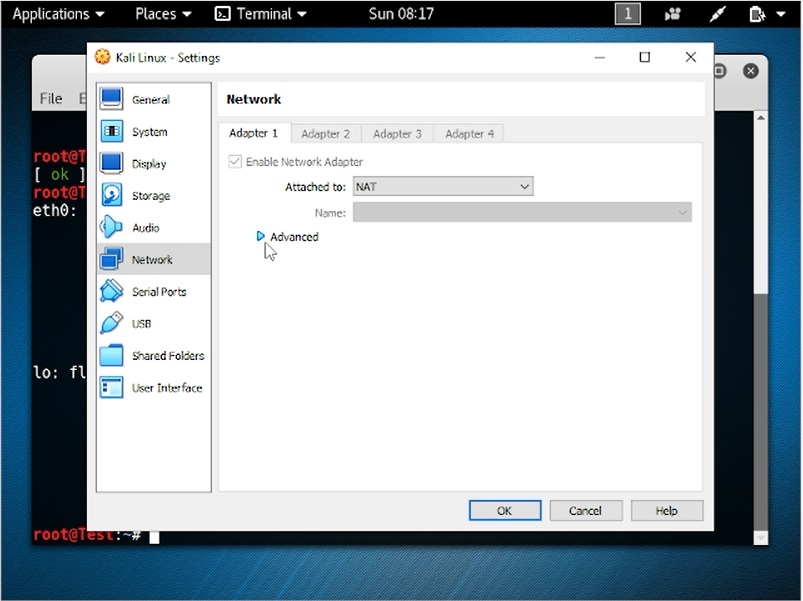
\includegraphics[width=0.85\linewidth]{figure//chapter5//lab5_1/vm_network.png}
    \caption{Network trong VirtualBox}
    \label{fig:enter-label}
\end{figure}

\newpage

\noindent {\bf{Bước 13:}} Ping \textbf{www.yahoo.com} để kiểm tra.

\begin{figure}[!htb]
    \centering
    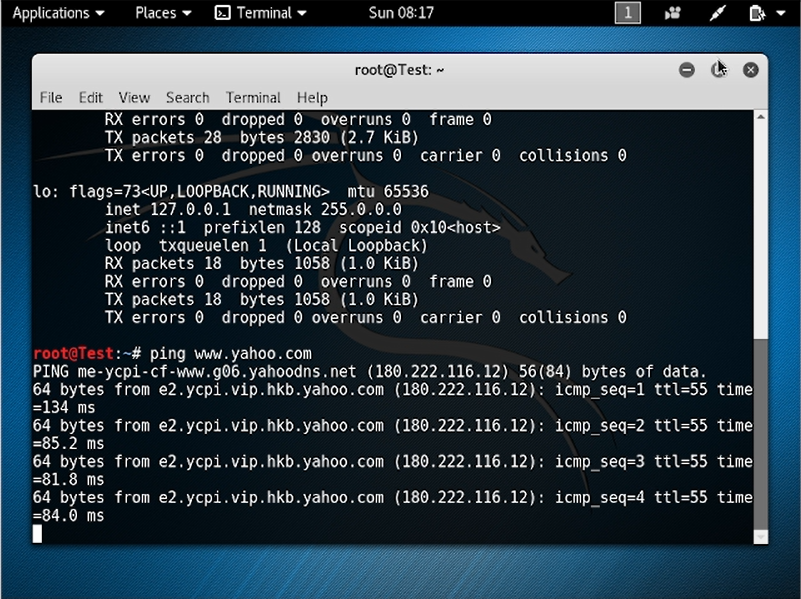
\includegraphics[width=0.85\linewidth]{figure//chapter5//lab5_1/ping_yahoo.png}
    \caption{Ping Yahoo}
    \label{fig:enter-label}
\end{figure}

\noindent {\bf{Bước 14:}} Chạy ứng dụng \textbf{ZenMap} trong \textbf{Application/Information Gathering}.

\begin{figure}[!htb]
    \centering
    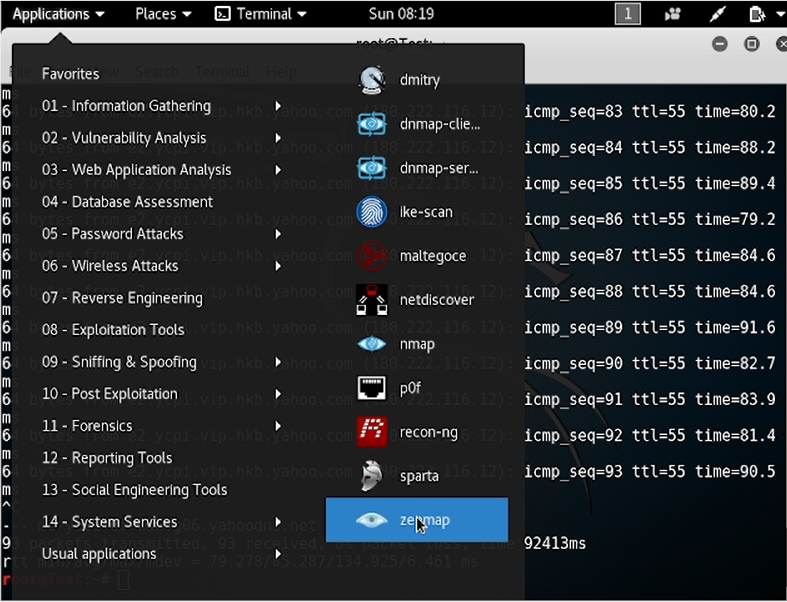
\includegraphics[width=0.85\linewidth]{figure//chapter5//lab5_1/zenmap.png}
    \caption{Chạy ứng dụng Zenmap}
    \label{fig:enter-label}
\end{figure}

\noindent {\bf{Bước 15:}} Ở phần \textbf{Target}, nhập \textbf{uet.vnu.edu.vn}. Sau đó chọn \textbf{Scan}.

\begin{figure}[!htb]
    \centering
    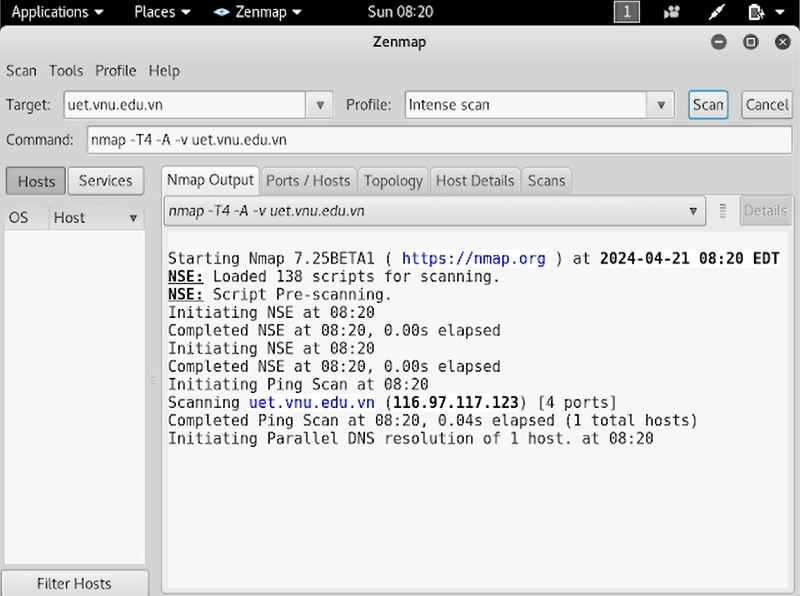
\includegraphics[width=0.85\linewidth]{figure//chapter5//lab5_1/scan-site.png}
    \caption{Scan uet.vnu.edu.vn}
    \label{fig:enter-label}
\end{figure}

\noindent {\bf{Bước 16:}} Chọn \textbf{Topology}. Tại đây, ta sẽ thấy các lần nhảy để tới được địa chỉ web đó.

\begin{figure}[!htb]
    \centering
    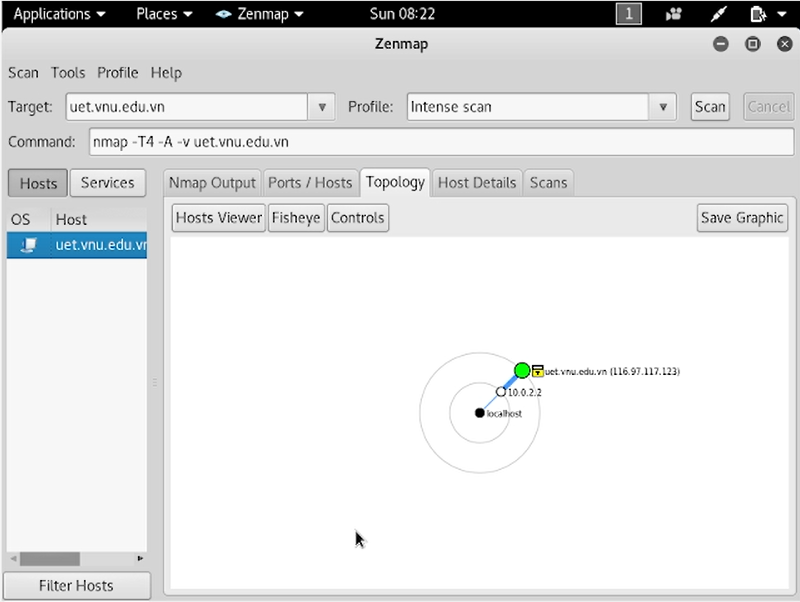
\includegraphics[width=0.85\linewidth]{figure//chapter5//lab5_1/topology.png}
    \caption{Màn hình Topology}
    \label{fig:enter-label}
\end{figure}

\newpage

\noindent {\bf{Bước 17:}} Mở \textbf{Nmap Output} và kiểm tra thêm các output.

\begin{figure}[!htb]
    \centering
    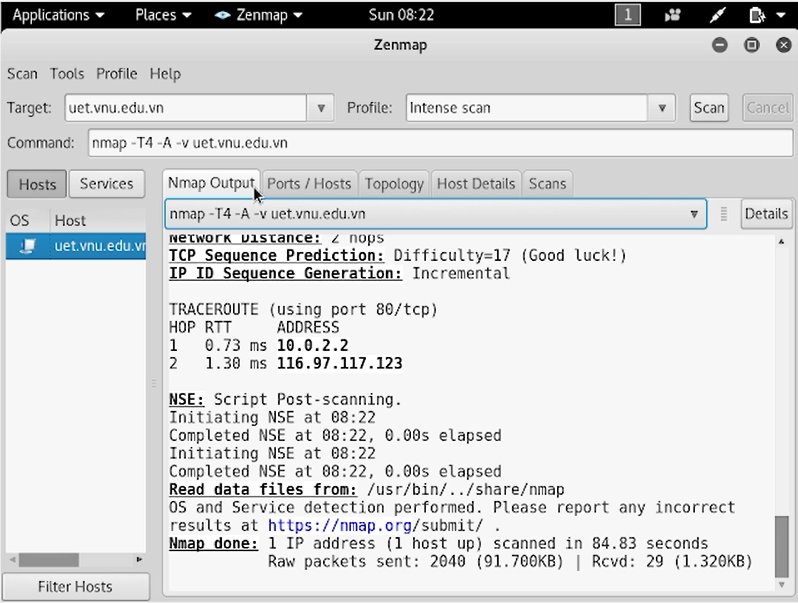
\includegraphics[width=0.85\linewidth]{figure//chapter5//lab5_1/nmap-output.png}
    \caption{Nmap Output}
    \label{fig:enter-label}
\end{figure}

\subsection{Review Questions}

\noindent Câu 1: 

B: BackTrack.

\noindent Câu 2: True.

\noindent Câu 3: 

D: GVim.

\noindent Câu 4:

C: 64.

\noindent Câu 5:

D: ls /etc.
